\section{ASHPMP 系统}
如图~\ref{F:1} 所示, ASHPMP 系统由压缩机、热管散热器、节流阀、蒸发器和管道组成。热管散热器、节流阀、蒸发器和管道组成。制冷剂从压缩机流出,进入 8 组冷凝器,这些冷凝器与热管共同构成热管散热器。热管散热器(HPR)。
每台设备都向室内释放热能、从而提高室内空气温度。

ASHPMP 系统的主要优点如下:
\begin{itemize}
    \item HPR 全部串联,安装和维护都很方便。
    \item 没有水箱、水泵和水管,不存在结霜风险。HPR 可以将热量迅速传递到室内,从而带来更加舒适惬意的供暖体验。
\end{itemize}

图~\ref{F:2} 显示了 HPR 的详细结构。如图~\ref{F:2a} 所示, HPR 由三大部分组成: 上收集管、下收集管和带散热片的热管。在下收集管中,如图~\ref{F:2b} 所示,由一个制冷剂入口管和出口管、一个压力表和一个制冷剂充注管,充注管作为维修阀门,用于抽真空和添加工作介质。冷凝管束插入其中。

为了降低成本,使用铝来制作 HPR。热管程度为 \qty{1.04}{m}, 高度为 \qty{0.8}{m},直径为 \qty{0.028}{m}。尺寸参数见图~\ref{F:3a},热管照片见图~\ref{F:3b}。

\begin{figure}[htbp]
	\centering
	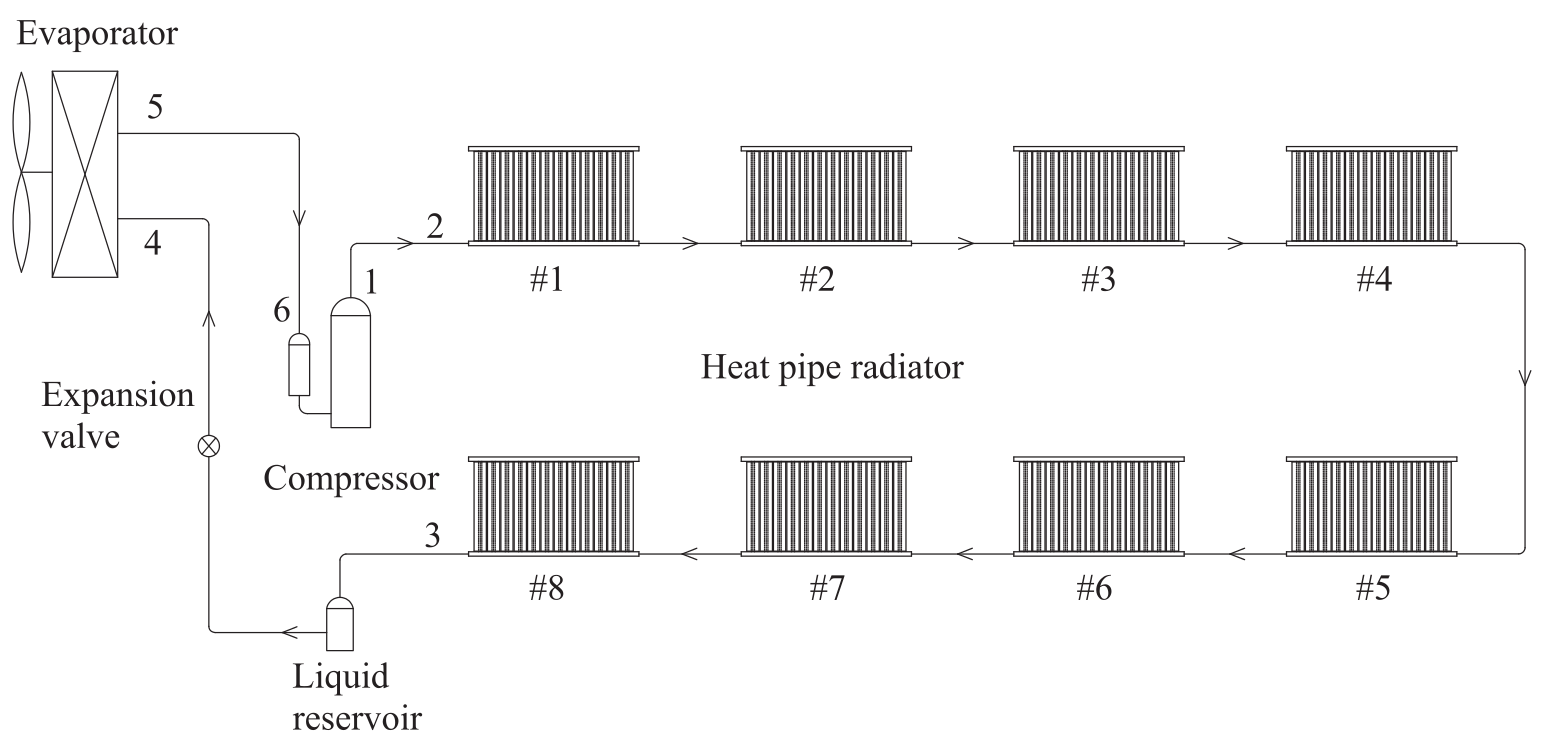
\includegraphics[width=0.7\textwidth]{picture/picture_1}
	\caption{ASHPMP 系统}
	\label{F:1}
\end{figure}

\begin{figure}[htbp]
\centering  %图片全局居中
\subfigure[HPR 结构参数]{
\label{F:2a}
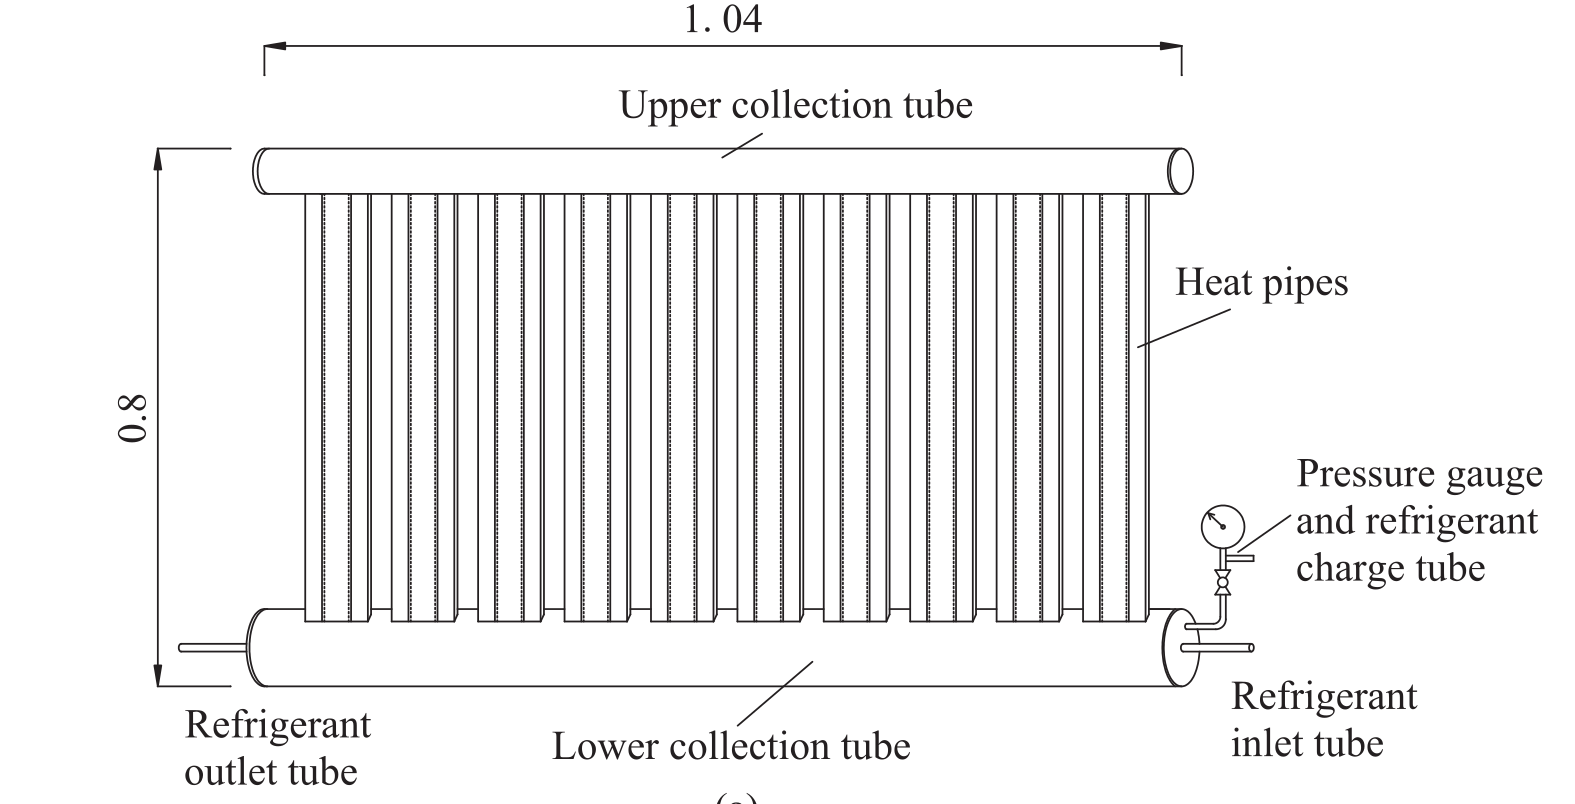
\includegraphics[width=0.7\textwidth]{picture/picture_2_a}}

\subfigure[下收集管的结构]{
\label{F:2b}
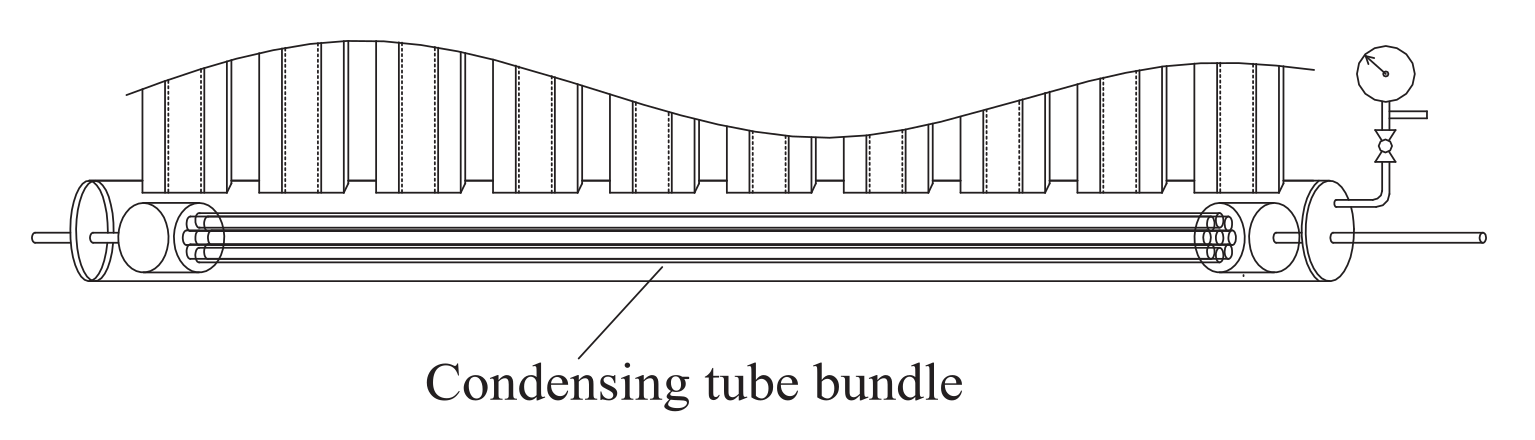
\includegraphics[width=0.7\textwidth]{picture/picture_2_b}}
\caption{HPR 和 冷凝器结构}
\label{F:2}
\end{figure}

\section{分析模型}
热泵冷凝器的热量通过强制对流传递给底部的热管制冷剂,然后通过液体和蒸汽空间传递给整个热管主体。最后,热量通过热管外表面的自然对流和辐射释放到室内空间中,
\begin{equation}\label{E:1}
	A = \frac{Q'_{r}}{h_c (t_f - T_i)} 
\end{equation}
其中,$Q'_r$ 为每根热管的散热量 $(\unit{\kW})$;$A$ 为表面积 $(\unit{\m^2)}$;$h_c$ 为复合传热系数 $(\unit{\kW/(\m^2\K)} )$;$t_f$ 是表面温度 $(\unit{\degreeCelsius})$;$T_i$ 是室温 $(\unit{\degreeCelsius})$。

冷凝管束中的单根管子的长度计算公式为:
\begin{equation}\label{E:2}
	l = 1000 Q'_r \frac{\ln (d_o/d_i)}{2 \pi n \lambda \Delta t} 
\end{equation}
其中,$\Delta t$ 为铜管内外表面温差$(\unit{\degreeCelsius})$; $d_o$为铜管外径$(\unit{\m})$, $\lambda$为铜管导热系数 $(\unit{\W/(\m\K)})$; $l$ 为铜管长度 $(\unit{\m})$; $n$ 为铜管数量。

管壁两侧的传热温差已知,传热面积可根据公式~\ref{E:1} 已知管壁两侧的传热温差,则传热面积可根据公式~\ref{E:2}。如图~\ref{F:4a} 所示,在每根热管的下部收集管中插入 9 根直径为$\qty{0.008}{\m} $的铜管。下收集管的直径为$\qty{0.04}{\m} $,厚度为$\qty{0.003}{\m}$。如图~\ref{F:4a} 所示。冷凝器与图~\ref{F:4b} 显示了与 HPR 相结合的冷凝器的照片。表~\ref{T:1} 概述了 HPR 的主要结构尺寸。

\begin{figure}[h]
\centering  %图片全局居中
\subfigure[热管尺寸参数]{
\label{F:3a}
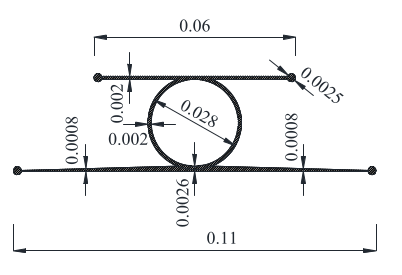
\includegraphics[width=0.3\textwidth]{picture/picture_3_a}}
\subfigure[热管照片]{
\label{F:3b}
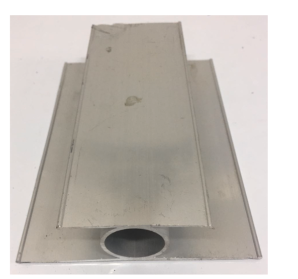
\includegraphics[width=0.3\textwidth]{picture/picture_3_b}}
\caption{热管尺寸与照片}
\label{F:3}
\end{figure}

\begin{figure}[h]
\centering  %图片全局居中
\subfigure[HPR 和 冷凝器的结构尺寸]{
\label{F:4a}
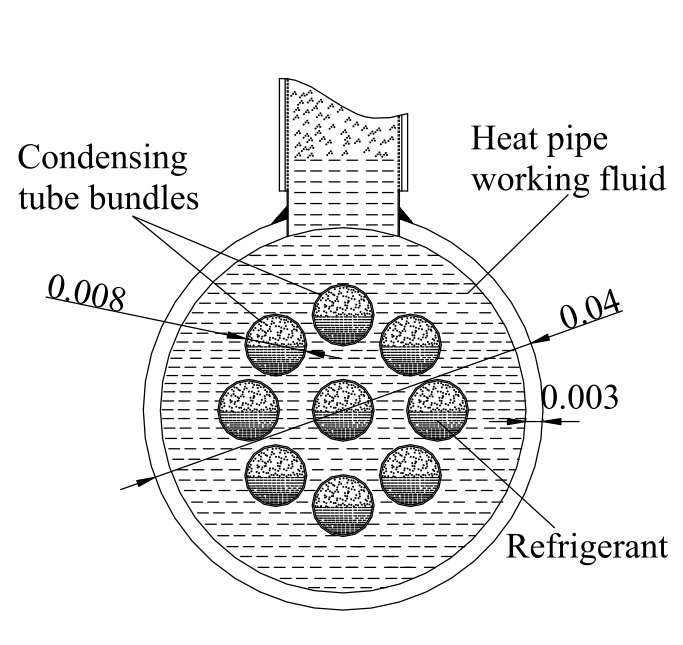
\includegraphics[width=0.3\textwidth]{picture/picture_4_a}}
\subfigure[配有 HPR 的冷凝器照片]{
\label{F:4b}
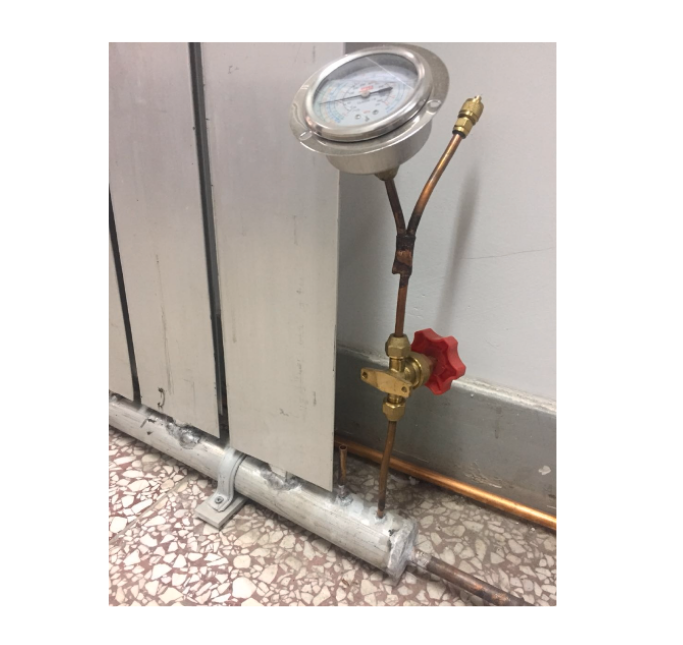
\includegraphics[width=0.3\textwidth]{picture/picture_4_b}}
\caption{HPR 与冷凝器的结构尺寸与照片}
\label{F:4}
\end{figure}

\begin{table}[ht]
\centering
\caption{主要尺寸结构}
\begin{tabular}{@{}lllllll@{}}
\toprule
宽度   & 高度  & 行号 & 尺寸    &       & 厚度    &       \\ \midrule
\qty{1.04}{\m} & \qty{0.8}{\m} & \qty{10}{\m} & 上下冷凝管 & 热管    & 上下冷凝管 & 热管    \\
     &     &    & \qty{0.04}{\m}   & \qty{0.028}{\m} & \qty{0.003}{\m} & \qty{0.002}{\m}  \\ \bottomrule
\end{tabular}
\label{T:1}
\end{table}

\section{实验设备}
新设备在中国北京进行了测试。如图~\ref{F:5} 所示试验室面积约为$\qty{25}{\m^2} $。压缩机排出的高温高压压缩机排出的高温高压蒸汽进入室内的 HPRs,再将热量传入室内。进而将热量传递到室内。热泵工作流体的热量工作流体的热量通过 HPR 散失。起初,制冷剂的状态可能保持不变,例如在 HPR \#1 中。在 HPR \#1 之后、温度降低的热泵制冷剂进入HPR \#2,继续通过 HPR 散热。此时,如果此时,如果第二台室内机的面积足够大,制冷剂将变成两相,并进入 HPR \#2。变成两相,进入 HPR \#3。同样,进入 \#4、\#5,直到最后一组。依次进入最后一组。当制冷剂从最后一个室内机流出时、工作介质是典型的过冷液体。

热管工作流体为 R134a。主要参数如每块热管的压力、室内外温度、空气侧进出口温度、室内室温等、室内室外温度、空气侧进出口温度、室内室温等主要参数。测量。为了研究系统中的压力分布,一定数量的压力传感器被安装在每个 HPRs 中,如图~\ref{F:5} 所示。

图~\ref{F:6} 展示了 ASHPMP 系统的照片,表~\ref{T:2} 列出了实验系统的规格。

压缩机的额定功率为$\qty{21}{\kW} $,工作流体为 R410A,由直流变频电机驱动。电机驱动,其频率在$\qty{0}{\hertz}$~\textasciitilde~$\qty{120}{\hertz} $之间变化。温度传感器设置在液态制冷剂管上,即膨胀阀之前的位置。当压缩机运行时,其转速由该温度点的设定值控制。当前温度低于设定温度时,压缩机转速会增加,当前温度低于设定温度时,压缩机转速会降低。当当前温度接近设定温度时,压缩机转速会降低。在一定的逻辑下,压缩机的速度根据当前温度和设定温度之间的差值来调节压缩机的转速。最后,最终控制温度温度波动范围很小。

压力传感器(不确定度 $\pm 5\%$)被用于测量热泵和热管的制冷剂压力。Pt100 温度传感器(不确定度 $\pm 5\%$)被用来测量空气和制冷剂温度。空气和制冷剂温度。液体管路中有一个质量流量计液体管路中装有质量流量计,可直接获得制冷剂的流量质量。不确定度 $\pm 5\%$ 的功率计用于监测压缩机的输入功率。压缩机的输入功率。加热能力Q $\unit{\kW} $和制热 COP 的不确定性可通过以下公式计算得出。仪器仪器和传播的不确定性总结如表~\ref{T:3}。

\begin{equation}\label{E:3}
	COP = \frac{Q}{W'} = \frac{m'(h_2 - h_3)}{W'} = f'(m',p_2,t_2,p_3,t_3,W')
\end{equation}

$m'$是制冷剂的质量流量$\unit{\kg/\s} $, $p_2, p_3$是制冷剂在图~\ref{F:5} 点 2 和 3 的压力$\unit{\MPa} $;$t_2, t_3$图~\ref{F:5} 点2 和 3 的制冷剂温度$\unit{\degreeCelsius} $; $h_2, h_3$是图~\ref{F:5} 点 2 和 3的焓$\unit{\kJ/\kg} $; $W'$是功率输入$\unit{\kW} $。

\begin{equation}\label{E:4}
	u_Q = \sqrt{(\frac{\partial f}{\partial m'} u_{m'})^2 + (\frac{\partial f}{\partial t_2} u_{t2})^2 + (\frac{\partial f}{\partial t_3} u_{t3} )^2+ (\frac{\partial f}{\partial p_2} u_{p2})^2 + (\frac{\partial f}{\partial t_2} u_{p3} )^2}
\end{equation}

\begin{equation}\label{E:5}
	u_{cop} = \sqrt{(\frac{\partial f}{\partial m'} u_{m'})^2 + (\frac{\partial f}{\partial t_2} u_{t2})^2 + (\frac{\partial f}{\partial t_3} u_{t3} )^2+ (\frac{\partial f}{\partial p_2} u_{p2})^2 + (\frac{\partial f}{\partial t_2} u_{p3} )^2 + (\frac{\partial f}{\partial W'} u_{w'})^2}
\end{equation}

\begin{equation}\label{E:6}
	u_{rel,Q} = \frac{u_Q}{Q} u_{rel,COP} = \frac{u_{cop}}{COP} 
\end{equation}

\begin{figure}[htbp]
	\centering
	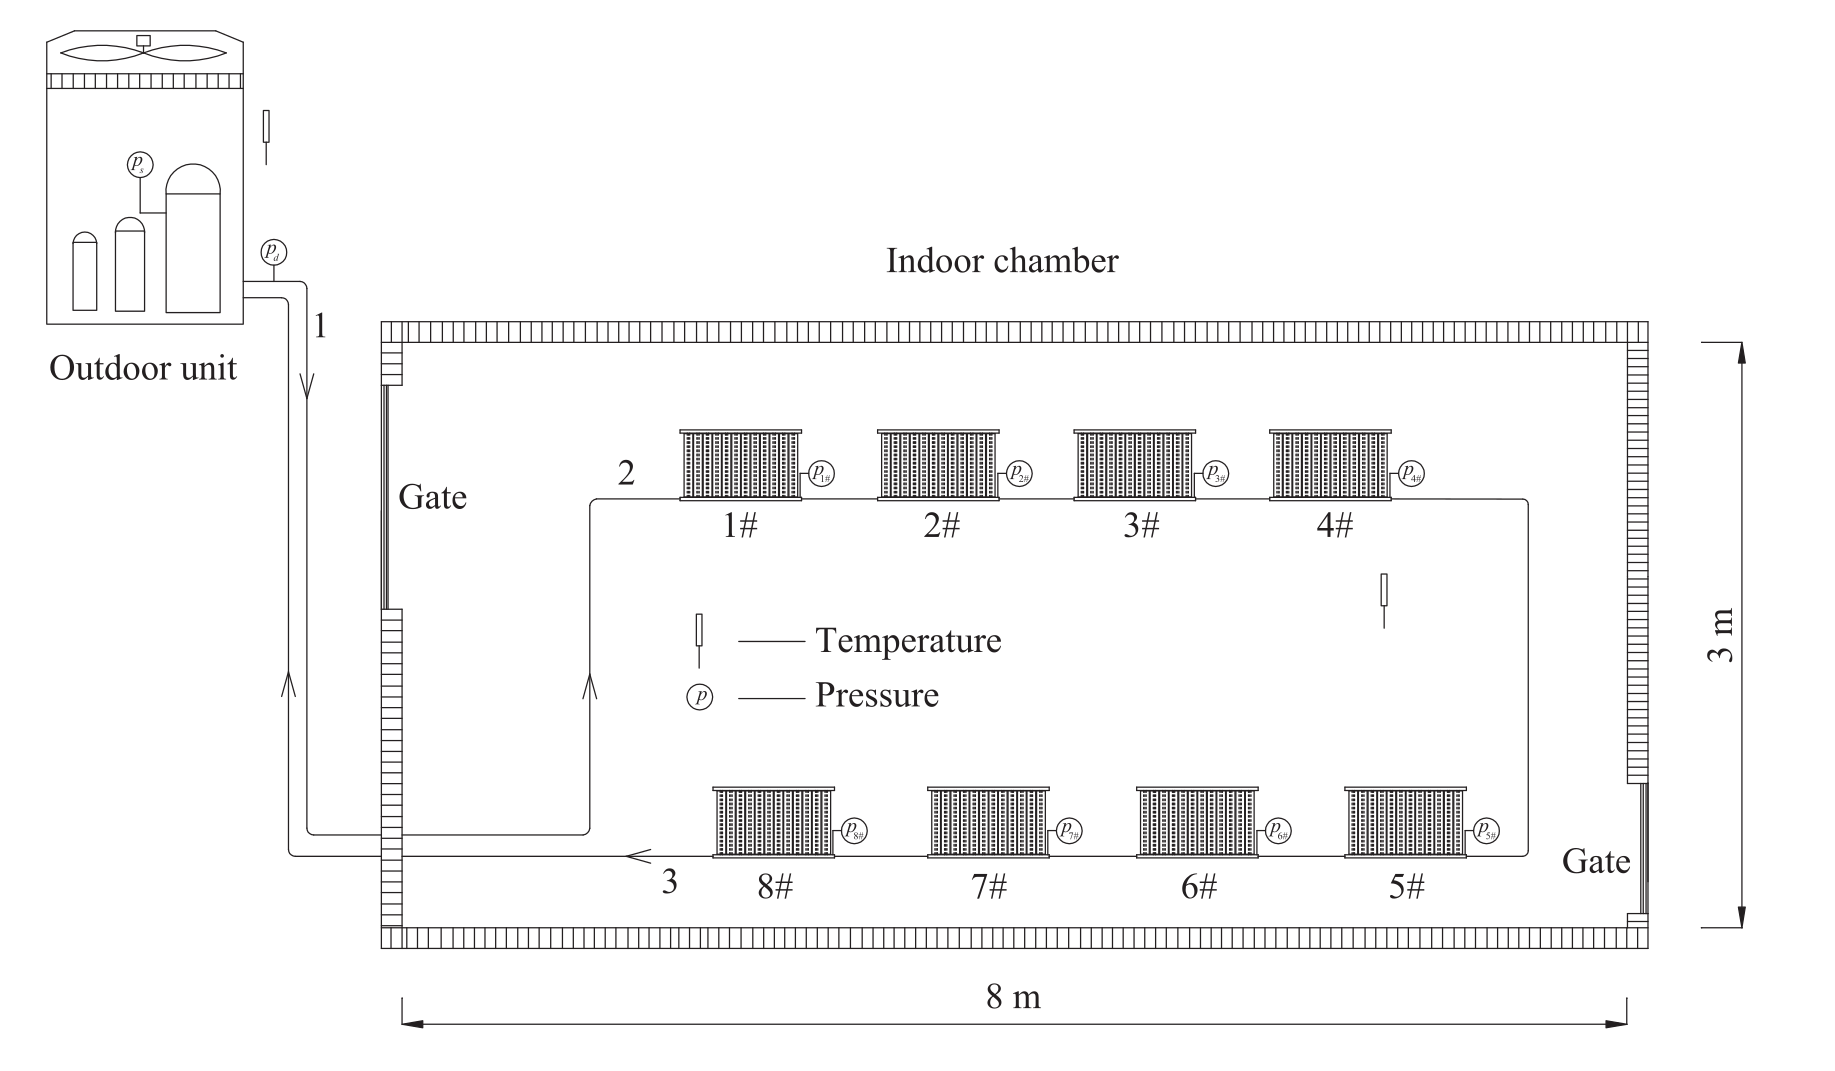
\includegraphics[width=0.7\textwidth]{picture/picture_5}
	\caption{原生测试系统示意图}
	\label{F:5}
\end{figure}

\begin{figure}[h]
\centering  %图片全局居中
\subfigure[外部单元]{
\label{F:6a}
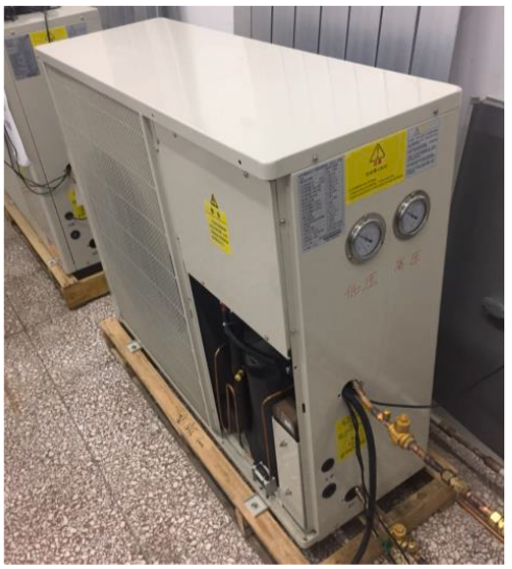
\includegraphics[width=0.3\textwidth]{picture/picture_6_a}}
\subfigure[内部单元]{
\label{F:6b}
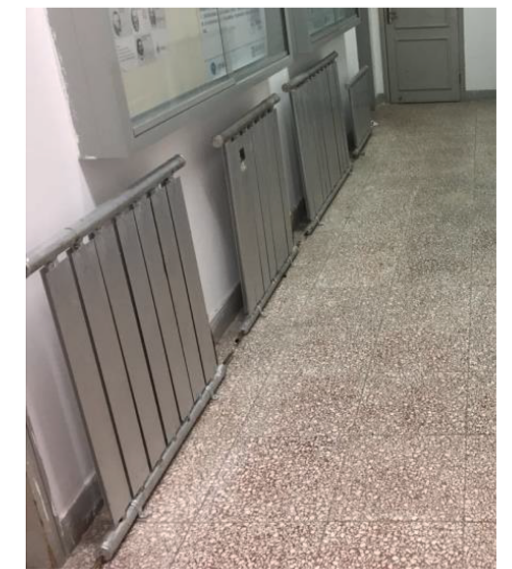
\includegraphics[width=0.3\textwidth]{picture/picture_6_b}}
\caption{ASHPMP 系统照片}
\label{F:6}
\end{figure}

\begin{table}[ht]
	\centering
	\caption{ASHPMP 系统特性}
	\begin{tabular}{@{}ll@{}}
		\toprule
		参数 	& 值/细节 \\ \midrule
		压缩机  & \\
		~压缩机类型  & 滚动活塞 \\
		~输入功率$\unit{\kW} $  & 0 \textasciitilde $\qty{3}{\kW} $ \\
		~制冷剂  & R410A \\
		EEV  & \\
		~模型  & CAREL $E^2 V$ \\
		室外热交换  & \\
		~类型  & 铜管/铝鳍片\\
		~额定容量 $\unit{\kW}$  & 8 \\
		~数量  & 1 \\
		室内交换器  & \\
		~类型  & HPR\\
		~额定容量 $\unit{\kW}$  & 1.2 \\
		~数量  & 8 \\
		~制冷剂  & R134a \\ \bottomrule
	\end{tabular}
	\label{T:2}
\end{table}

\begin{table}[ht]
	\centering
	\caption{实验参数的不确定性}
	\begin{tabular}{@{}llll@{}}
		\toprule
		传感器 & 精确度 & 全量程 & 模型 \\ \midrule
		温度传感器 & $\pm\qty{0.15}{\degreeCelsius} $ & - & Pt100 \\
		压力传感器 & $\pm 0.5\%$ 全量程 & $\qty{4.0}{\MPa} $ & Huba \\
		流量计 & $\pm 0.2\%$ 全量程 & $\qty{250}{\g/\s} $ & Shouke \\
		电力采集单元 & $\pm 0.5\%$ 全量程 & $\qty{10}{\kW} $ & DZFC-1 \\
		数据采集器 & $\pm 0.2\%$ 全量程 & - & HP34972A \\
		加热能力 & $2.9\%$ & & \\
		热 COP & $3.9\%$ & & \\ \bottomrule
	\end{tabular}
	\label{T:3}
\end{table}
